%%% The main file. It contains definitions of basic parameters and includes all other parts.

%% Settings for single-side (simplex) printing
% Margins: left 40mm, right 25mm, top and bottom 25mm
% (but beware, LaTeX adds 1in implicitly)
\documentclass[12pt,a4paper]{report}
\setlength\textwidth{145mm}
\setlength\textheight{247mm}
\setlength\oddsidemargin{15mm}
\setlength\evensidemargin{15mm}
\setlength\topmargin{0mm}
\setlength\headsep{0mm}
\setlength\headheight{0mm}
% \openright makes the following text appear on a right-hand page
\let\openright=\clearpage

%% Settings for two-sided (duplex) printing
% \documentclass[12pt,a4paper,twoside,openright]{report}
% \setlength\textwidth{145mm}
% \setlength\textheight{247mm}
% \setlength\oddsidemargin{14.2mm}
% \setlength\evensidemargin{0mm}
% \setlength\topmargin{0mm}
% \setlength\headsep{0mm}
% \setlength\headheight{0mm}
% \let\openright=\cleardoublepage

%% Generate PDF/A-2u
\usepackage[a-2u]{pdfx}

%% Character encoding: usually latin2, cp1250 or utf8:
\usepackage[utf8]{inputenc}

%% Prefer Latin Modern fonts
\usepackage{lmodern}

%% Further useful packages (included in most LaTeX distributions)
\usepackage{amsmath}        % extensions for typesetting of math
\usepackage{amsfonts}       % math fonts
\usepackage{amsthm}         % theorems, definitions, etc.
\usepackage{bbding}         % various symbols (squares, asterisks, scissors, ...)
\usepackage{bm}             % boldface symbols (\bm)
\usepackage{graphicx}       % embedding of pictures
\usepackage{fancyvrb}       % improved verbatim environment
\usepackage{natbib}         % citation style AUTHOR (YEAR), or AUTHOR [NUMBER]
\usepackage[nottoc]{tocbibind} % makes sure that bibliography and the lists
			    % of figures/tables are included in the table
			    % of contents
\usepackage{dcolumn}        % improved alignment of table columns
\usepackage{booktabs}       % improved horizontal lines in tables
\usepackage{paralist}       % improved enumerate and itemize
\usepackage{xcolor}         % typesetting in color
\usepackage{todonotes}
%%% Basic information on the thesis

% Thesis title in English (exactly as in the formal assignment)
\def\ThesisTitle{Optimal choice of scenario tree using Reinforcement learning}

% Author of the thesis
\def\ThesisAuthor{Bc. Jakub Vondráček}

% Year when the thesis is submitted
\def\YearSubmitted{2022}

% Name of the department or institute, where the work was officially assigned
% (according to the Organizational Structure of MFF UK in English,
% or a full name of a department outside MFF)
\def\Department{Department of Probability and Mathematical Statistics}

% Is it a department (katedra), or an institute (ústav)?
\def\DeptType{Department}

% Thesis supervisor: name, surname and titles
\def\Supervisor{doc.~RNDr.~Ing.~Miloš~Kopa,~Ph.D.}

% Supervisor's department (again according to Organizational structure of MFF)
\def\SupervisorsDepartment{Department of Probability and Mathematical Statistics}

% Study programme and specialization
\def\StudyProgramme{Probability, mathematical statistics and econometrics}
\def\StudyBranch{\textcolor{red}{study branch}}

% An optional dedication: you can thank whomever you wish (your supervisor,
% consultant, a person who lent the software, etc.)
\def\Dedication{%
Dedication.
}

% Abstract (recommended length around 80-200 words; this is not a copy of your thesis assignment!)
\def\Abstract{%
Abstract.
}

% 3 to 5 keywords (recommended), each enclosed in curly braces
\def\Keywords{%
{key} {words}
}

%% The hyperref package for clickable links in PDF and also for storing
%% metadata to PDF (including the table of contents).
%% Most settings are pre-set by the pdfx package.
\hypersetup{unicode}
\hypersetup{breaklinks=true}

% Definitions of macros (see description inside)
%%% This file contains definitions of various useful macros and environments %%%
%%% Please add more macros here instead of cluttering other files with them. %%%

%%% Minor tweaks of style

% These macros employ a little dirty trick to convince LaTeX to typeset
% chapter headings sanely, without lots of empty space above them.
% Feel free to ignore.
\makeatletter
\def\@makechapterhead#1{
  {\parindent \z@ \raggedright \normalfont
   \Huge\bfseries \thechapter. #1
   \par\nobreak
   \vskip 20\p@
}}
\def\@makeschapterhead#1{
  {\parindent \z@ \raggedright \normalfont
   \Huge\bfseries #1
   \par\nobreak
   \vskip 20\p@
}}
\makeatother

% This macro defines a chapter, which is not numbered, but is included
% in the table of contents.
\def\chapwithtoc#1{
\chapter*{#1}
\addcontentsline{toc}{chapter}{#1}
}

% Draw black "slugs" whenever a line overflows, so that we can spot it easily.
\overfullrule=1mm

%%% Macros for definitions, theorems, claims, examples, ... (requires amsthm package)

\theoremstyle{plain}
\newtheorem{thm}{Theorem}
\newtheorem{lemma}[thm]{Lemma}
\newtheorem{claim}[thm]{Claim}

\theoremstyle{plain}
\newtheorem{defn}{Definition}

\theoremstyle{remark}
\newtheorem*{cor}{Corollary}
\newtheorem*{rem}{Remark}
\newtheorem*{example}{Example}

%%% An environment for proofs

\newenvironment{myproof}{
  \par\medskip\noindent
  \textit{Proof}.
}{
\newline
\rightline{$\qedsymbol$}
}

%%% An environment for typesetting of program code and input/output
%%% of programs. (Requires the fancyvrb package -- fancy verbatim.)

\DefineVerbatimEnvironment{code}{Verbatim}{fontsize=\small, frame=single}

%%% The field of all real and natural numbers
\newcommand{\R}{\mathbb{R}}
\newcommand{\N}{\mathbb{N}}

%%% Useful operators for statistics and probability
\DeclareMathOperator{\pr}{\textsf{P}}
\DeclareMathOperator{\E}{\textsf{E}\,}
\DeclareMathOperator{\var}{\textrm{var}}
\DeclareMathOperator{\sd}{\textrm{sd}}

%%% Transposition of a vector/matrix
\newcommand{\T}[1]{#1^\top}

%%% Various math goodies
\newcommand{\goto}{\rightarrow}
\newcommand{\gotop}{\stackrel{P}{\longrightarrow}}
\newcommand{\maon}[1]{o(n^{#1})}
\newcommand{\abs}[1]{\left|{#1}\right|}
\newcommand{\dint}{\int_0^\tau\!\!\int_0^\tau}
\newcommand{\isqr}[1]{\frac{1}{\sqrt{#1}}}

%%% Various table goodies
\newcommand{\pulrad}[1]{\raisebox{1.5ex}[0pt]{#1}}
\newcommand{\mc}[1]{\multicolumn{1}{c}{#1}}


% Title page and various mandatory informational pages
\begin{document}
%%% Title page of the thesis and other mandatory pages
%%% Title page of the thesis

\pagestyle{empty}
\hypersetup{pageanchor=false}
\begin{center}

\centerline{\mbox{
\includegraphics[width=166mm]{../img/logo-en.pdf}}}

\vspace{-8mm}
\vfill

{\bf\Large MASTER THESIS}

\vfill

{\LARGE\ThesisAuthor}

\vspace{15mm}

{\LARGE\bfseries\ThesisTitle}

\vfill

\Department

\vfill

{
\centerline{\vbox{\halign{\hbox to 0.45\hsize{\hfil #}&\hskip 0.5em\parbox[t]{0.45\hsize}{\raggedright #}\cr
Supervisor of the master thesis:&\Supervisor \cr
\noalign{\vspace{2mm}}
Study programme:&\StudyProgramme \cr
\noalign{\vspace{2mm}}
Study branch:&\StudyBranch \cr
}}}}


\vfill

% Zde doplňte rok
Prague \YearSubmitted

\end{center}

\newpage

%%% Here should be a bound sheet included -- a signed copy of the "master
%%% thesis assignment". This assignment is NOT a part of the electronic
%%% version of the thesis. DO NOT SCAN.

%%% A page with a solemn declaration to the master thesis

\openright
\hypersetup{pageanchor=true}
\pagestyle{plain}
\pagenumbering{roman}
\vglue 0pt plus 1fill

\noindent
I declare that I carried out this master thesis independently, and only with the cited
sources, literature and other professional sources. It has not been used to obtain another
or the same degree.

\medskip\noindent
I understand that my work relates to the rights and obligations under the Act No.~121/2000 Sb.,
the Copyright Act, as amended, in particular the fact that the Charles
University has the right to conclude a license agreement on the use of this
work as a school work pursuant to Section 60 subsection 1 of the Copyright~Act.

\vspace{10mm}

\hbox{\hbox to 0.5\hsize{%
In \hbox to 6em{\dotfill} date \hbox to 6em{\dotfill}
\hss}\hbox to 0.5\hsize{\dotfill\quad}}
\smallskip
\hbox{\hbox to 0.5\hsize{}\hbox to 0.5\hsize{\hfil Author's signature\hfil}}

\vspace{20mm}
\newpage

%%% Dedication

\openright

\noindent
\Dedication

\newpage

%%% Mandatory information page of the thesis

\openright

\vbox to 0.5\vsize{
\setlength\parindent{0mm}
\setlength\parskip{5mm}

Title:
\ThesisTitle

Author:
\ThesisAuthor

\DeptType:
\Department

Supervisor:
\Supervisor, \SupervisorsDepartment

Abstract:
\Abstract

Keywords:
\Keywords

\vss}

\newpage

\openright
\pagestyle{plain}
\pagenumbering{arabic}
\setcounter{page}{1}


%%% A page with automatically generated table of contents of the master thesis

\tableofcontents

%%% Each chapter is kept in a separate file
\chapter*{Introduction}
\addcontentsline{toc}{chapter}{Introduction}
Stochastic programming is a branch of mathematical optimization that allows to account for uncertain parameters when solving mathematical programs, which led to the widespread adoption of stochastic programming in fields such as finance, transportation, scheduling and telecommunications. 

This makes it a very powerful tool, which however comes at a significant computational cost. Due to the fact that the random parameters may follow a continuous distribution, approximating such distributions by a discrete set of scenarios is necessary to even be able to formulate the model and also to be able to solve it in finite time. Even more demanding are so called multistage programs, which allow multiple decision periods. To be able to solve multistage programs, the scenarios approximating the continuous distributions in every stage are arranged in a scenario tree. The structure of this tree is very important for the obtained solution, as a tree that is very simple may not approximate the underlying distribution correctly, while a tree that is too complex suffers from extensive computational costs. 

This is the main idea of this thesis -- to discover whether it is possible to predict a scenario tree structure that is optimal with regard to the objective function and also potentially with regard to the complexity of the scenario tree. To solve this problem, we propose an experiment to train a reinforcement learning agent using the solutions of a mean-CVaR model calculated using scenario trees generated from historical financial data. 

Chapters \ref{chap1}, \ref{chap2} and \ref{chapter3} provide the necessary theory for Multistage stochastic programming, the mean CVaR model and Reinforcement learning respectively. The mean CVaR model formulated in Section \ref{section:endofhorizoncvar_scenario_formulation}, while certainly not novel, is of our own design.  The main contribution of this thesis is Chapter \ref{chapter4}, the pinnacle of this thesis, where we implement the experiment described above and analyse the results. To the best of our knowledge, such an experiment has not been proposed in the literature. Also a notable contribution is the compilation and standardization of notation for several machine learning algorithms in Chapter \ref{chapter3} from multiple different sources.
\chapter{Stochastic programming}


%
%Structure of thesis:
%Introduction
%Multistage stochastic programming problems
%-multistage idea, nonanticipativity constraints, deterministic equivalent
%-curse of dimensionality
%-scenario trees 
%    -moment matching, geometric brownian motion + clustering
%Risk measures
%-VaR, CVaR, minimisation, L shaped method, reformulating as a multistage program
%Reinforcement learning
%-introduction, comparison to other types (supervised etc), no loss function - inspiration from learning of animals and men
%-Basic idea
%-Multiarmed bandits
%Study
%-Formulation of the whole problem (idea of thesis)
%    -Idea how to evaluate
%    -Penalisation of result using complexity of tree with a hyperparameter - explain reasoning why we should penalise the result - why are complex scenario trees bad (long computation time, ...)?
%-Data
%-Computational problems, complexity, how long does solving each small problem take
%-Results of the study
%

%Stochastic programming 
%-Framework to model problems which involve uncertainty
%-Optimization problem where some or all parameters are uncertain in contrast to deterministic optimization
%-the goal is to find a solution which is feasible for all such data and optimal in some sense
%-Stochastic programming models are similar in style but take advantage of the fact that probability distributions governing the data are known or can be estimated
%-The goal is to find some policy that is feasible for all (or almost all) the possible parameter realizations
%and optimizes the expectation of some function of the decisions and the random variables
%-Areas where stochastic programming is used
%	-financial planning, airline scheduling, transportation (truck routes, daily milk delivery with random demand), management of power systems
	
In this chapter, we give an introduction to the theory of stochastic programming with particular focus on multistage linear programs. Most of the content in this chapter is based on the material covered in \cite[Chapter 1]{stochasticprogrammingbible}, \cite[Chapters 1-3]{stochasticprogrammingbible2009} and \cite[Part 2]{dupacovastochasticprogramming}.
\todo{Add more meat here}

\section{Basic definitions}
\begin{defn}{Mathematical program in $\R^n$ \cite[p. 107]{dupacovastochasticprogramming}}. \\
\label{def:MathematicalProgramDef}
Let $p,m,n \in \N$. A mathematical program in $\R^n$ is defined as
\begin{equation*}
\mathrm{min} \{f(\mathbf{x}), \mathbf{x} \in \mathbf{M}\},
\end{equation*}
where $\mathbf{M} \subset \R^n$ and $f$ is a real function. The function $f$ is called the objective function and the set $\mathbf{M}$ is called the set of feasible solutions. 
This set is usually defined by constraints as follows:
\begin{equation*}
	\mathbf{M} = \{\mathbf{x} \in \R^n: h_j(\mathbf{x})=0, \, j=1,\dots,p, \, g_k(\mathbf{x}) \leq 0, k=1,\dots,m \},
\end{equation*}
where $h_j,j=1,\dots,p$ and $g_k, k=1,\dots,m $ are real functions.
\end{defn}
If $\mathbf{M}=\R^n$ and all functions in Definition~\ref{def:MathematicalProgramDef} are linear, we call the problem a \textit{Linear program}.
Furthermore, if any of the functions mentioned in Definition~\ref{def:MathematicalProgramDef} depend on parameters, we call the problem a \textit{Parametric program}. If any of the parameters are uncertain \textcolor{red}{(random variables)}\todo{Is random variable ok here? I assume it is, just for check.}, we call the problem a \textit{Stochastic program}.


However, the Stochastic program is not well defined. Consider the Definition~\ref{def:MathematicalProgramDef} and let $\Omega$ be a non-empty set, $\mathcal{F}$ be a  $\sigma$-algebra on $\Omega$, $\omega \in \Omega$ and $\mathcal{P}$ be a probability measure on $(\Omega, \mathcal{F})$, leading to a probability space $(\Omega, \mathcal{F}, \mathcal{P})$. In the context of a Stochastic program, the function $f$ does not depend on $\mathbf{x}$ only, but also on the realisation of $\omega$. This leads to a nonsensical definition, as for different realisations of $\omega$, the optimal value may be different. The standard way to handle this problem is to consider minimisation of expected value of the function $f$:

\begin{equation*}
\mathrm{min} \{\mathbb{E}\left[f(\mathbf{x}, \omega)\right], \mathbf{x} \in \mathbf{M}\},
\end{equation*}
where $\mathbb{E}$ is the expected value operator defined with respect to the probability measure $\mathcal{P}$. \todo{Are these definitions (mostly the probability measure stuff) correct?}


\section{Multistage stochastic programming}
The stochastic programming paradigm allows to make an optimal decision with regard to the expectation, but only for one decision period. This is a considerable limitation, which can be overcome by extending the notion of a \textit{Stochastic program} to a \textit{Multistage stochastic program}. 

\subsection{Notation and general idea}
This section is heavily inspired by \cite[Section 3.3.]{stochasticprogrammingbible}.
Following the notation established there, consider the following sequence of events
\begin{equation*}
\begin{gathered}
\mathrm{Decision} \, \, x_1 
\\
\downarrow
\\
\mathrm{Observation} \,\, \xi_2
\\
\downarrow
\\
\mathrm{Decision} \,\, x_2 
\\
\downarrow
\\
\mathrm{Observation} \,\, \xi_3
\\
\downarrow
\\
\vdots
\\
\downarrow
\\
\mathrm{Observation} \,\, \xi_T
\\
\downarrow
\\
\mathrm{Decision} \,\, x_T,
\end{gathered}
\end{equation*}
where $T$ is the number of stages, $x=(x_1,\dots,x_T)$ is called the decision process ($x_1$ is a non-random vector of variables), $\xi = (\xi_2,\dots,\xi_T)$ is a stochastic data process ($\xi_1$ is assumed to be known and deterministic). The decision process $x$ represents the decisions made at each stage (i.e. for a portfolio allocation problem, $x_t$ may be a random vector of proportions of some assets in a portfolio at some intermediate stage\todo{is this clear? Maybe rewrite}) and $\xi_T$ is a random vector representing the data proccess in the last stage (i.e. it may be a vector of yearly asset returns). Furthermore, the probability distribution of $\xi$ is assumed to be known.
\subsection{Nonanticipativity constraints}
Both processes $x$ and $\xi$ are random and thus depend on the realised $\omega \in \Omega$. In order for the program to be well defined, the decision process $x$ must not take into account future observations of either 
$\xi$ or decisions $x$, but only the past and present. This is formalised by the so called nonanticipativity constraints, which assure that the $x_t$ may depend only on $(x_1,\dots,x_{t-1})$ and $(\xi_1,...,\xi_{t})$.

\begin{defn}{Nonanticipativity constraints} \cite[Section 3.3.]{stochasticprogrammingbible}. \\
\label{def:nonanticipativity constraints}
The decision process $x$ is termed nonanticipative if
\begin{equation*}
x_t=\mathbb{E}\left[x_t|\xi_1,\dots,\xi_t \right], t=1,\dots,T,
\end{equation*}
or equivalently, if $\mathcal{F}_t$ is the $\sigma$-algebra generated by $(\xi_1,\dots,\xi_t)$, then $x_t(\omega)$\todo{should ($\omega$) be here?} must be measurable with respect to $\mathcal{F}_t$, where $\mathcal{F}_1 \subset \mathcal{F}_2 \subset \dots \subset \mathcal{F}_T \subset \mathcal{F}$.
\end{defn}

\subsection{Scenario trees}
\subsubsection{Methods for generation of scenario trees}
\subsection{Curse of dimensionality}
\section{Risk measures}

\chapter{Risk measures}
When investing, the investor has to make a decision whether to trade certainty for potentially higher profit in the future. If he would invest in a risk free asset, then some small positive return is guaranteed. Investing in a risky asset can yield significantly higher returns, but of course there is no free lunch. The potentially higher returns are compensated for by the fact that the investor may incur loss. To quantify the degree of riskiness of such assets, several risk measures have been introduced over time.
In the following, we will follow mainly \cite{leoppold_risk_measures} and \cite[p. 275-278]{cornuejols_tutuncu_2006} if not specified otherwise.

\begin{defn}{Measure of risk} \\
Let $\mathcal{V}$ be the set of real random variables. A risk measure $\rho$ maps the random variable to a real value, i.e. $\rho: \mathcal{V} \rightarrow \R$.
\end{defn}

Let $\mathcal{R}$ be a random variable representing returns of a portfolio. In the last century, one of the most popular risk measures was the variance of returns of an asset, used famously in the Nobel Prize winning model in \cite{markowitz}, where a porfolio selection model was formulated that maximised the expected return while minimising the variance in returns. To be precise, variance in returns is defined as
\begin{equation*}
\sigma^2=E(\mathcal{R} - \mathbb{E}\mathcal{R} )^2.
\end{equation*}
Although at the time the achievement of the Markowitz model was groundbreaking, the use of variance as a risk measure has been a subject of debate. The problem is that variance is symmetric and does not take into account the tails of the distribution of $\mathcal{R}$. To handle the symmetry problem, another risk measure was proposed, the semivariance defined as
\begin{equation*}
\gamma=\mathbb{E}(max(\mathcal{L} - \mathbb{E}\mathcal{L},0))^2=\mathbb{E}(max(-\mathcal{R} + \mathbb{E}\mathcal{R},0))^2,
\end{equation*}
where $\mathcal{L}=-\mathcal{R}$ is the loss random variable.
%Notice that both variance and semivariance yield the same result whether the random variable $\mathcal{R}$ represents returns or losses of the portfolio.

Let us now introduce the notion of a \textit{coherent measure of risk}, which was developed in \cite[Defintion 2.4.]{coherent_measures_of_risk} and aims to provide a set of properties that a “nice” risk measure should satistfy.
\begin{defn}{Coherent measure of risk} \\
Let $\mathcal{V}$ be the set of real random variables. We say that a risk measure $\rho: \mathcal{V} \rightarrow \R$ is coherent if it satisfies the following properties:
\begin{enumerate}
	\item Monotony: $X, Y \in \mathcal{V}, X(\omega) \leq Y(\omega) \, \forall \omega \in \Omega \implies \rho(X) \geq \rho(Y)$.
	\item Subadditivity: $X, Y, X+Y \in \mathcal{V} \implies \rho(X+	Y) \leq \rho(X) + \rho(Y)$.
	\item Positive homogenity: $X \in \mathcal{V}, h \geq 0, hX \in \mathcal{V} \implies \rho(hX)=h\rho(X)$.
	\item Translation equivariance: $X \in \mathcal{V}, a \in \R \implies \rho(X+a)=\rho(X)-a$.
\end{enumerate}
\end{defn}
The properties have a quite nice interpretation. The monotony property implies that a portfolio $Y$ that is more favourable in all possible scenarios should have smaller risk compared to the less favourable portfolio $X$. The subadditivity property pertains to the notion of diversification, as it says that if we combine two portfolios $X$ and $Y$, the resulting combined portfolio should not be riskier than the portfolios separately. The positive homogenity property pertains to the notion of leverage -- if we leverage our portfolio by some factor $h\geq0$, the risk should change proportionally to $h$. Last is the property of translation equivariance, which says that increasing the value of portfolio by risk free $a$, the risk profile is decreased by $a$. \todo{is this translation equivariance property ok? I think it is, just to check.} Unfortunately, neither variance not semivariance are coherent risk measures.

Let us now introduce another risk measure, the \textit{value at risk}.
Using the notation developed in \cite{cornuejols_tutuncu_2006}, let $f(x,\Upsilon)$ be a loss function of a vector $x$ which may be considered as a portfolio and a random vector $\Upsilon$ which represents the unknown returns or other random aspects influencing the distribution of loss and denote the loss random variable $\mathcal{L}(x,\Upsilon)=f(x,\Upsilon)$. We assume that the probability distribution of $\Upsilon$ is known and for simplicity that $\Upsilon$ has a probability density $p(y)$. The cumulative distribution function of $\mathcal{L}(x,\Upsilon)$ is then defined as
\begin{equation*}
\Psi(x,\upsilon)=\int_{f(x,y) \leq \upsilon} p(y) \, \mathrm{d}y.
\end{equation*}

\begin{defn}{Value at risk \cite[p. 275]{cornuejols_tutuncu_2006}.}  \\
Let $\alpha$ be the chosen confidence level and let $\mathcal{L}(x,\Upsilon)$ have the meaning of loss distribution as defined above with the cumulative distribution function $\Psi(x,\upsilon)$. Then the value at risk $VaR_{\alpha}(x)$ is defined as
\begin{equation*}
VaR_{\alpha}(x)=q_{\alpha}(x)
\end{equation*}
where $q_{\alpha}(x)=\mathrm{min}\{\upsilon \in \R: \Psi(x,\upsilon) \geq \alpha \}$ is the lower $\alpha$ quantile of distribution of $\mathcal{L}(x,\Upsilon)$. $\alpha$ is usually chosen as $0.95$ or $0.99$.
\end{defn}
\todo{Here I present the definition of VaR for continuous distributions (so that I don't have to deal with upper and lower quantiles and upper and lower VaR. Is this ok or should I make it explicit and add the definitions for discrete distributions?}

\begin{figure}
  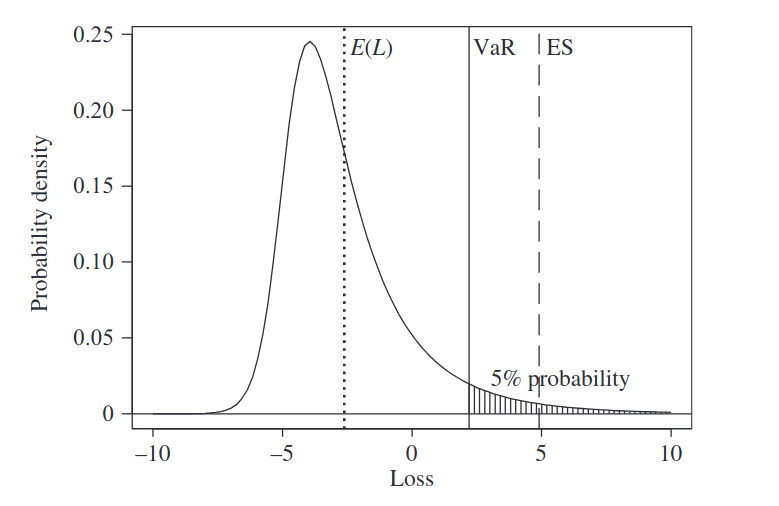
\includegraphics[width=\linewidth]{../img/VaR_CVaR_graph_theory.png}
  \caption{Illustration of $VaR_{0.95}$ and $CVaR_{0.95}$ (where $CVaR_{0.95}$ is labeled as ES). Image sourced from \cite[Figure 2.2.]{mcneil2015quantitative}. \textcolor{red}{TODO: generate the figure myself}}
  \label{fig:VaR_CVaR_graph_theory}
\end{figure}


Value at risk also comes with several advantages and disadvantages. While it is simple to understand and globally accepted by regulators, it is not coherent in general (the subadditivity requirement is not fulfilled), it doesn't quantify the losses exceeding $VaR_{\alpha}(x)$ and it is not convex (this makes it hard to optimize a portfolio with regard to value at risk).

Due to the aforementioned disadvantages of value at risk, another risk measure was considered.
Considering the expected loss exceeding the $VaR_{\alpha}(x)$ level leads to the notion of \textit{Conditional value at risk}. \todo{Add conditional value at risk.}

\begin{defn}{Conditional value at risk} 
\label{cvar_definition}
\\  
\cite[p. 275]{cornuejols_tutuncu_2006}
\\
Let $\alpha$ be the chosen confidence level and let $\mathcal{L}(x,\Upsilon)$ have the meaning of loss distribution as defined above and assume that $\mathbb{E}(\abs{\mathcal{L}(x,\Upsilon)})<\infty$. Then the conditional value at risk or expected shortfall $CVaR_{\alpha}(x)$ is defined as
\begin{equation}
CVaR_{\alpha}(x)=\frac{1}{1-\alpha}\int_{f(x,y) \geq VaR_{\alpha}(x)} f(x,y)p(y) \, \mathrm{d} y.
\end{equation}
\end{defn}
Compared to value at risk, conditional value at risk is a coherent risk measure (for the proof, see \cite[Example 2.26.]{mcneil2015quantitative}), but since value at risk is present in its definition, optimizing a portfolio with regard to conditional value at risk according to this definition suffers from many of the same problems as optimizing a portfolio with regard to value at risk. Therefore, a new method has been developed in \cite{Rockafellar2000OptimizationOC} that allows optimization of conditional value at risk without computing value at risk using linear programming.

\section{Minimising CVaR using scenarios}
In this section, we closely follow the exposition provided in \cite[p. 275-278]{cornuejols_tutuncu_2006}.
Let
\begin{equation}
\label{eq:cvar_approx}
F_{\alpha}(x,\gamma)=\gamma + \frac{1}{1-\alpha} \int_{f(x,y) \geq \gamma} (f(x,y)-\gamma)p(y) \, \mathrm{d}y.
\end{equation}
The function $F_{\alpha}(x,\gamma)$ has three important properties:
\begin{lemma}{Properties of $F_{\alpha}(x,\gamma)$ \cite[p. 276]{cornuejols_tutuncu_2006}.}
\label{lemma:properties_of_cvar_approx} 
\\
The following three properties hold for $F_{\alpha}(x,\gamma)$:
\begin{enumerate}
	\item It is a convex function of $\gamma$.
	\item $VaR_{\alpha}(x)=\underset{\gamma}{\mathrm{argmin}} \, F_{\alpha}(x,\gamma)$.
	\item $ CVaR_{\alpha}(x) = \underset{\gamma}{\mathrm{min}} \, F_{\alpha}(x,\gamma)$.
\end{enumerate}
\end{lemma}
\begin{proof}
For the proof, see \cite[Theorems 1 and 2]{Rockafellar2000OptimizationOC}
\end{proof}
\subsection{CVaR formulation}
If we want to choose a portfolio $x$ that minimises $CVaR_{\alpha}(x)$, we can now do so by minimising $F_{\alpha}(x,\gamma)$ over $x \in \mathcal{X}$ and $\gamma \in \R$ (where $\mathcal{X}$ is some set of portfolios) thanks to the third property in Lemma \ref{lemma:properties_of_cvar_approx}. Of course, Equation \ref{eq:cvar_approx} is not particularly suitable for numerical computations. In practice, as was explained in detail in Chapter \ref{chap1}, the distribution of $\Upsilon$ is approximated using scenarios $\gamma_s$ with associated probabilities $p_s, s=1,\dots,S$.

We can then calculate an approximation of $F_{\alpha}(x,\gamma)$ as
\begin{equation}
\label{eq:cvar_approx_approx}
\hat{F}_{\alpha}(x,\gamma)=\gamma + \frac{1}{1-\alpha} \sum_{s=1}^S  p_s \max (f(x,\gamma_s)- \gamma,0).
\end{equation}
We have arrived at the optimization problem
\begin{equation}
\label{eq:cvar_optim_first}
\underset{x \in \mathcal{X}, \gamma}{\min} \hat{F}_{\alpha}(x,\gamma)= \underset{x \in \mathcal{X}, \gamma}{\min} \gamma + \frac{1}{1-\alpha} \sum_{s=1}^S p_s \max (f(x,\gamma_s)-\gamma,0).
\end{equation}
A trick can be used to turn Equation \ref{eq:cvar_optim_first} into a linear programming problem. If we create new variables $z_s \geq 0$ such that $z_s \geq f(x,\gamma_s)-\gamma$, we can write:
\begin{alignat}{10}
& \underset{x \in \mathcal{X}, z_s \geq 0, \gamma}{\min}  \, \, \, && \gamma + \frac{1}{1-\alpha} \sum_{s=1}^S p_s z_s \\
&s.t. && \, z_s \geq f(x,\gamma_s)-\gamma, s=1,\dots,S
\end{alignat}
which is a linear programming problem.
\subsection{Mean-CVaR formulation}
In this section, we present a more precise formulation for practical use adopted from \cite{cvar_robust_mean_cvar_portfolio_optimization}, particularly when we want to choose a portfolio that minimises the conditional value at risk and also allows for controlling the minimum expected return or setting the degree of risk aversion.
\subsubsection*{Formulation with minimum expected return}
Let $x=(x_1,\dots,x_n)$ be a vector denoting of weights of each of $n$ assets in a portfolio and consider that $\mu=(\mu_1,\dots,\mu_n)$ is a random vector representing the returns of the assets. Consider $S$ scenarios, each with probability $p_s$ and let $r_s = (r_{1,s},\dots,r_{n,s})$ be the particular realisation of $\mu$ in scenario $s$ and let $r_0$ be the minimum required expected return. For simplicity, we do not allow short selling (condition $x_i \geq 0, i=1,\dots,n$). Then we can write
\begin{alignat}{10}
& \underset{x_i \geq 0 , z_s \geq 0, \gamma}{\min}  \, \, \, && \gamma + \frac{1}{(1-\alpha)} \sum_{s=1}^S p_s z_s, \label{cvar_expected_return}  \\
&s.t. && \, z_s \geq  -\sum_{i=1}^{n} x_i r_{i,s} -\gamma, s=1,\dots,S, \nonumber \\
&  && \sum_{i=1}^{n} x_i \bar{R_i} \geq r_0, \label{eq:cvar_expected_return:min_return_equation} \\
&  && \sum_{i=1}^{n} x_i = 1, \nonumber
\end{alignat}
where $\bar{R_i}=\sum_{s=1}^{S}p_s r_{i,s}$, which is still a linear programming problem. Equation \ref{eq:cvar_expected_return:min_return_equation} assures the minimal expected return.
\subsubsection*{Formulation using risk aversion}
Another equivalent formulation might be useful when the decision maker does not require a minimum expected return explicitly, but rather wants to set his risk aversion expectations. This can be achieved by introducing a risk aversion parameter $\lambda \geq 0$ and writing
\begin{alignat}{10}
& \underset{x_i \geq 0 , z_s \geq 0, \gamma}{\min}  \, \, \, && \sum_{i=1}^{n} x_i \bar{R_i} + \lambda \left( \gamma + \frac{1}{(1-\alpha)} \sum_{s=1}^S p_s z_s \right), \label{eq:cvar_risk_aversion} \\
&s.t. && \, z_s \geq  -\sum_{i=1}^{n} x_i r_{i,s} -\gamma, s=1,\dots,S, \nonumber \\
&  && \sum_{i=1}^{n} x_i = 1. \nonumber
\end{alignat}
\section{Minimising CVaR using scenarios in multistage setting}
In the multistage setting, the problem is a bit more complicated. Since the returns now do not occur at one single time but rather it is a sequence of returns, the notion of a risk measure must be extended accordingly. For the purposes of this thesis, we focus on the \textit{end of horizon $CVaR$}, for more advanced topics such as \textit{Nested $CVaR$ model} or \textit{Sum of $CVaR$ model}, we refer the reader to the summary in \cite[Section 1.4.]{kozmikv_phdthesis}.

\subsection{End of horizon CVaR}

\begin{defn}{End of horizon $CVaR$.} \\
Consider Definition \ref{cvar_definition}. If we consider the $CVaR$ calculated from the last stage (at the end of the investment horizon), we call it end of horizon $CVaR$.
\end{defn}
The definition of \textit{end of horizon $CVaR$} is very similar to the definition of regular $CVaR$, with the small difference that the multistage formulation now allows the decision maker to reallocate funds during the investment period (at the end of each stage). 

\subsubsection{End of horizon CVaR - scenario formulation}
We now extend Formulations \ref{cvar_expected_return} and \ref{eq:cvar_risk_aversion} to the multistage case. Consider we want to optimise a portfolio consisting of $n$ stocks over $T$ stages and consider a scenario tree with $S$ leaves (here we abuse notation and write sets $S=\{1,\dots,S\}$, $T=\{1,\dots,T\}$ and $I=\{1,\dots,n\})$. The problem \ref{cvar_expected_return} can then be reformulated as Equation \ref{eq:cvar_multistage_expected_return} by introducing variables $w_{t,s}$ which represent the wealth in scenario $s$ at time $t$ and $tot_s$ which is the total return in scenario $s$.

\begin{alignat}{10}
& \min \, \, \, && \gamma + \frac{1}{(1-\alpha)} \sum_{s=1}^S p_s z_s, \label{eq:cvar_multistage_expected_return}  \\
&s.t. && \, z_s \geq  -tot_s -\gamma, \forall s \in S \nonumber \\
&  && \sum_{s=1}^{S} p_s tot_s \geq r_0, \nonumber \\
& && w_{1,s}=1, \forall s \in S, \nonumber \\
& && w_{t,s}=\sum_{i=1}^{n} x_{i,t,s}, \forall s \in S, \forall t \in \{1,\dots,T-1\}, \label{eq:cvar_multistage_expected_return:wealth_distribution} \\
& && w_{t+1,s}=\sum_{i=1}^{n} r_{i,t,s} x_{i,t,s}, \forall s \in S, \forall t \in \{1,\dots ,T-1\}, \label{eq:cvar_multistage_expected_return:wealth_increases} \\
& && tot_s = \frac{w_{T,s}}{w_{1,s}}, \forall s \in S, \nonumber \\
& && z_s \geq 0, \forall s \in S, \nonumber \\
& && x_{i,t,s} \geq 0, \forall s \in S, \forall i \in I, \forall t \in \{1,\dots ,T-1\}, \nonumber \\
& && \gamma \in \R ,\nonumber \\
& && + \mathrm{nonanticipativity \, constraints}, \nonumber
\end{alignat}
The initial wealth $w_{1,s}$ is set to 1 and in each stage, the wealth increases by the returns obtained in the previous stage (Equation \ref{eq:cvar_multistage_expected_return:wealth_increases}) and is distributed again (Equation \ref{eq:cvar_multistage_expected_return:wealth_distribution}, at the end of the investment horizon we do not need to distribute the wealth into assets again). $r_{i,t,s}$ is the return obtained from stock $i$ at stage $t$ in scenario $s$ (we consider returns indexed by $t$ to occur at the end of stage $t$ (after the portfolio allocations $x_{i,t,s}$ are set), so that Equation \ref{eq:cvar_multistage_expected_return:wealth_increases} makes sense). The returns $r_{i,t,s}$ are of the form $1+r$ (where if the asset gained 6 percent, then $r_{i,t,s}=1.06$). This justifies Equation \ref{eq:cvar_multistage_expected_return:wealth_increases}. $tot_s \, \forall s \in S$ and $r_0$ are then again of the form $1+r$.

\begin{rem}
We do not include the nonanticipativity constraints in the above formulation, since they must be specified explicitly according to the structure of the scenario tree. To illustrate the explicit formulation of nonanticipativity constraints, consider Figure \ref{fig:balanced_scenario_tree}. In the context of the above problem, there are 6 scenarios ($111, 112, 113, 121, 122, 123$). For this illustration, let $\mathbf{x}_{t,s}$ be the vector of allocations to each assets at time $t$ and in scenario $s$. The nonanticipativity constraints now read:
\begin{alignat}{10}
& && \mathbf{x}_{t1,111}=\mathbf{x}_{t1,112}=\mathbf{x}_{t1,113}=\mathbf{x}_{t1,121}=\mathbf{x}_{t1,122}=\mathbf{x}_{t1,123} \nonumber \\
& && \mathbf{x}_{t2,111}=\mathbf{x}_{t2,112}=\mathbf{x}_{t2,113},\mathbf{x}_{t2,121}=\mathbf{x}_{t2,122}=\mathbf{x}_{t2,123}. \nonumber
\end{alignat}
\end{rem}
Similarly, the problem \ref{eq:cvar_risk_aversion} can then be reformulated as Equation \ref{eq:cvar_multistage_risk_aversion}:

\begin{alignat}{10}
& \min  \, \, \, &&\sum_{s=1}^{S} p_s tot_s + \lambda \left( \gamma + \frac{1}{(1-\alpha)} \sum_{s=1}^S p_s z_s \right), \label{eq:cvar_multistage_risk_aversion}  \\
&s.t. && \, z_s \geq  -tot_s -\gamma, \forall s \in S \nonumber \\
& && w_{1,s}=1, \forall s \in S, \nonumber \\
& && w_{t,s}=\sum_{i=1}^{n} x_{i,t,s}, \forall s \in S, \forall t \in \{1,\dots ,T-1\}, \label{eq:cvar_multistage_expected_return:wealth_distribution_risk_aversion} \\
& && w_{t+1,s}=\sum_{i=1}^{n} r_{i,t,s} x_{i,t,s}, \forall s \in S, \forall t \in \{1,\dots ,T-1\}, \label{eq:cvar_multistage_expected_return:wealth_increases_risk_aversion} \\
& && tot_s = \frac{w_{T,s}}{w_{1,s}}, \forall s \in S, \nonumber \\
& && z_s \geq 0, \forall s \in S, \nonumber \\
& && x_{i,t,s} \geq 0, \forall s \in S, \forall i \in I, \forall t \in \{1,\dots ,T-1\}, \nonumber \\
& && \gamma \in \R ,\nonumber \\
& && + \mathrm{nonanticipativity \, constraints}, \nonumber
\end{alignat}
where $\lambda \geq 0$ is a risk aversion parameter and the nonanticipativity constraints would again need to be provided explicitly according to the structure of the scenario tree.

\chapter*{Conclusion}
\addcontentsline{toc}{chapter}{Conclusion}


%%% Bibliography
%%% Bibliography (literature used as a source)
%%%
%%% We employ bibTeX to construct the bibliography. It processes
%%% citations in the text (e.g., the \cite{...} macro) and looks up
%%% relevant entries in the bibliography.bib file.
%%%
%%% The \bibliographystyle command selects, which style will be used
%%% for references from the text. The argument in curly brackets is
%%% the name of the corresponding style file (*.bst). Both styles
%%% mentioned in this template are included in LaTeX distributions.

\bibliographystyle{plainnat}    %% Author (year)
% \bibliographystyle{unsrt}     %% [number]

\renewcommand{\bibname}{Bibliography}

%%% Generate the bibliography. Beware that if you cited no works,
%%% the empty list will be omitted completely.

\bibliography{bibliography}

%%% If case you prefer to write the bibliography manually (without bibTeX),
%%% you can use the following. Please follow the ISO 690 standard and
%%% citation conventions of your field of research.

% \begin{thebibliography}{99}
%
% \bibitem{lamport94}
%   {\sc Lamport,} Leslie.
%   \emph{\LaTeX: A Document Preparation System}.
%   2nd edition.
%   Massachusetts: Addison Wesley, 1994.
%   ISBN 0-201-52983-1.
%
% \end{thebibliography}


%%% Figures used in the thesis (consider if this is needed)
\listoffigures

%%% Tables used in the thesis (consider if this is needed)
%%% In mathematical theses, it could be better to move the list of tables to the beginning of the thesis.
\listoftables

%%% Abbreviations used in the thesis, if any, including their explanation
%%% In mathematical theses, it could be better to move the list of abbreviations to the beginning of the thesis.
\chapwithtoc{List of Abbreviations}

%%% Attachments to the master thesis, if any. Each attachment must be
%%% referred to at least once from the text of the thesis. Attachments
%%% are numbered.
%%%
%%% The printed version should preferably contain attachments, which can be
%%% read (additional tables and charts, supplementary text, examples of
%%% program output, etc.). The electronic version is more suited for attachments
%%% which will likely be used in an electronic form rather than read (program
%%% source code, data files, interactive charts, etc.). Electronic attachments
%%% should be uploaded to SIS and optionally also included in the thesis on a~CD/DVD.
%%% Allowed file formats are specified in provision of the rector no. 72/2017.
\appendix
\chapter{Attachments}

\section{First Attachment}

\openright
\end{document}
